\section{Data Description}
\label{sec:rawData}
As it has been shown in \cite{Hong:2013:TAS:2528282.2528302} correlation values 
Data obtained from the PIR sensors is binary in nature. 1 indicates occupancy and 0 indicates non occupancy. \\
First step to determine the sensor location is to cluster the neighboring sensors together. If two sensors are physically close to each other, and people move from sensing region of one sensor to the other the correlation value must be high.
Since neighboring sensors observe the same event, correlation value between the neighboring sensors should be high. So we compute the correlation coefficient of the raw data. To calculate the correlation between the binary data we use  the formula as given by equation \ref{eq:binCorr}.
\begin{equation}
\label{eq:binCorr}
correlation ratio = \frac{a^2}{p_1\times p_2}
\end{equation}
a : number of 1’s in the same position in both the data.\\
P1: number of 1’s in data set 1.\\
P2:number of 1’s in dataset 2.\\
The result were not good, with correlation between neighboring sensors being as low as 0.08 as shown in the Figure \ref{fig:rawData}.


\section{Feature Extraction}
\label{ref:feature}
As seen in section \ref{sec:rawData} raw data analysis gives poor correlation values for the raw sensor data, hence we look at extracting features from the raw data set and computing correlation values for the feature of the sensor data. One of the feature that we consider is the energy of the signal. Energy for a binary data stream can be computed using equation \ref{eq:energyEq}.
Energy feature is computed on 36 sample windows of pir sensor data with 50\% overlapping between consecutive windows. At sampling frequency of 100ms, window length of 36 corresponds to 3.6s data.
The energy of bianry signal x(n) is computed as given in \ref{eq:energyEq}.\\
\begin{equation}
\label{eq:energyEq}
E_s = {\sum_{n=-\infty}^{\infty}{|x(n)|}^2}
\end{equation}
TODO: Explain why energy is used.
Energy of PIR signal along with giving the indication that the region is occupied it also gives information about the extent of activity in the region of occupancy. To differentiate between the neighboring nodes and non neighboring nodes we use Pearson correlation coefficient given by \ref{eq:corrcoeff}. 



\begin{figure}%
\centering

\subfloat[Croos correlation values of raw sensors data]{{\includegraphics[width=5cm]{./pics/raw_data_correlation.pdf}}}%
\label{fig:rawData}

\qquad
\subfloat[Croos correlation values for energy of the sensors data]{\includegraphics[width=4cm]{./pics/energy_correlation.pdf}}%
\label{fig:energyData}
\caption{Correlation values}
\end{figure}

By setting a threshold of 0.23 we can differentiate between the neighboring and non neighboring nodes. Now the goal is to use the correlation coefficients of the energy data to determine the sensor location. A straight forward way to determine the sensor location would be to perform a brute force test and place the sensor on the grid and calculate the sum of the correlation coefficients between the neighboring sensors. Brute force for a 8 sensor grid means checking 8! possible arrangement.  Which is a small number but as the number of sensors increases it is not possible to compute brute force. Therefore we need to to cutdown the possible arrangemetns that are supposed to be checked. For that we propose an algorithm as explained in the next section.

\section{Algorithm}
The blackbox description of the algorithm is as shown in the figure \ref{fig:algorithm}. 
\begin{figure}
\includegraphics[scale=0.5]{./pics/algorithm.png}
\caption{High level overview of the Algorithm}
\label{fig:algorithm}
\end{figure}
The inputs required for the algorithm are:
\begin{itemize}
\item  Coordinates of the grid vertices.
\item Pir sensor data.
\item   Pir sensors field of view.
\end{itemize}
The algorithm outputs the sensor coordinates. 
First step in determining the sensor locations is to identify the neighboring sensors for every sensors. 
Definitions :
Neighboring sensors- Two sensors are said to be neighbors if they have overlapping field of view. 
Grid adjacency Matrix: We represent the sensor grid in the form of a adjacency matrix. Two vertices of the grid are adjacent if the distance between them is less than twice the radius of the sensors field of view.
\[
GAM_{i,j} = 
\begin{cases}
1, & if d_{i,j} < 2r \forall i \ne j\\
0, & otherwise\\
\end{cases}
	\]


 For which we use the correlation coefficients value between all the sensors. The main challenge in identifying the neighbors from a given correlation matrix is choosing a threshold which can differentiate between neighboring and non neighboring nodes. One of the things that we can be sure about from the correlation coefficient matrix is that the maximum cross correlation coefficient is always between the neighboring nodes. Hence we obtain a maximum spanning tree for the correlation coefficient.
\section{Maximum Spanning Tree over correlation coefficient Matrix}
To obtain the maximum spanning tree over correlation coefficient matrix we use the Prim's algorithm\cite{BLTJ:BLTJ1515}. Prim's algorithm compute the minimum spanning tree. As we require maximum spanning tree we negate the correlation values and apply Prims's algorithm. We randomly choose one of the sensor nodes as the root and obtain the maximum spanning tree. The properties of the maximum spanning tree are :
\begin{itemize}
\item The maximum spanning tree covers all the nodes.
\item An edge exists between the nodes which have a strong correlation coefficient.
\end{itemize}
By computing the maximum spanning tree we partially identify the neighboring nodes. The next step is to identify the remaining neighboring sensor nodes and place the sensors on the grid. As we know the grid structure(coordinates of the vertices ), we map this tree onto the grid. 

\begin{figure}%

\raggedright
\subfloat[A 4 $\times$ 2 grid]{
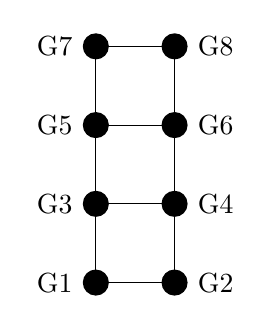
\begin{tikzpicture}
\draw(0,0) grid(1,3);
\draw(0,0) node[circle,fill=black,label=left:G1]{};
\draw(1,0) node[circle,fill=black,label=right:G2]{};
\draw(0,1) node[circle,fill=black,label=left:G3]{};
\draw(1,1) node[circle,fill=black,label=right:G4]{};
\draw(0,2) node[circle,fill=black,label=left:G5]{};
\draw(1,2) node[circle,fill=black,label=right:G6]{};
\draw(0,3) node[circle,fill=black,label=left:G7]{};
\draw(1,3) node[circle,fill=black,label=right:G8]{};
\end{tikzpicture}}%
\quad
\begingroup
\captionsetup[subfigure]{width=\widthof{Maximum spanning tree for the sensor correlation matrix}}
\centering
\subfloat[Maximum spanning tree for the sensor correlation matrix  ]{
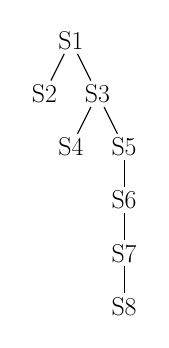
\begin{tikzpicture} [scale=.45,transform shape] 
\node{\huge S1}
child{node{ \huge S2}}
child{node{\huge S3} 
	child{node{\huge S4}} 
	child{node{\huge S5}
    	child{node{\huge S6}
        	child{node{\huge S7}
           child{node{\huge S8}
            }
            }
            }
    	}
    };

 \end{tikzpicture}}
\endgroup
\label{fig:gridTree}
\end{figure}




This process helps us to identify the neighbors as well as the sensors location on the grid. The mapping of a spanning tree on to the graph is a classic problem of graph monomorphism. 
We define graph monomorphism on graph G and H as: \\
A function $ \phi:V(G) \rightarrow  V(H)$ is monomorphic from G to H if   $  \forall v,w \in E_G \Rightarrow (\phi((v),\space \phi(w)) \in E_H.$\\
In our case we have a spanning tree H which we want to map it to the grid graph G.
\section{Graph Monomorphism}
\subsection{VF2}

In this section we explain graph monomorphism and give a brief description about VF2 algorithm.\\
Pseudo-code \\
\begin{figure}
\begin{algorithm}[H]
\textbf{Procedure} Match(s)\\
\textbf{INPUT:}  an intermediate state s; the initial state $s_0$ has $M(s_0)=\emptyset$\\
\textbf{OUTPUT:} the mappings between two graphs>\;
\textbf{Match(s)}\\
 \textbf{IF} M(s) covers all the nodes of $G_2$ \textbf{THEN}\\
               \textbf{OUTPUT} M(s)\\
\textbf{ELSE}\\
                 Compute the set P(s) of the pairs of candidates for inclusion in M(s)\\
\textbf{FOREACH} (n,m) $\in$ P(s)\\
\textbf{IF} F(s,n,m) \textbf{THEN}\\
	Compute the state s' obtained by adding (n,m) to M(s)\\
\textbf{CALL} Match(s')\\
\textbf{ENDIF}\\
\textbf{ENDFOREACH}\\
Restore data structure\\
\textbf{ENDIF}\\
\caption{VF2 algorithm}

\end{algorithm}
\label{fig:VF2}
\end{figure}
Consider the graphs shown in figure \ref{fig:gridTree} representing 

% VF2 explanation 
VF2 algorithm is an algorithm to solve subgraph isomorphism problem. VF2 is a depth search first algorithm. It uses recursive backtracking technique. A process of matching 
the grid graph G to its spanning tree consists of determining a mapping M which associate nodes of $Grid(G)$ with nodes of the Tree(T) and vice versa, with some constraints.
Mapping is expressed as a set of pairs (n,m) with (n $\in$ G and m $\in$ T). 
In VF2 algorithm the process of finding a mapping is represented as a State Space Representation (SSR). Each state s of the matching process can be associated to a partial mapping solution M(s),
which contains only a subset of M. A transition from current state(s) to the next state(s') represents the addition of a mapping (n,m) to the state s.

VF2 algorithm introduces a set of rules which helps to prune the number of possible SSR that needs to be checked before obtaining the a valid mapping. Figure \ref{fig:VF2} gives a high-lvel description of the VF2 algorithm.
There are 2 important functionalities in the algorithm one is the generation of possible mappings and the other is the checking of the validity of the mapping.

\subsection{Computation of candidate pair set P(s)}
This section explains the method to compute the candidate pair set P(S) for an undirected graph G and T. 
Set $T_1(s)$ and $T_2(s)$ are defined for Graph G and T respectively, representing the nodes which are neighbors of the set of nodes including in the partial mapping state(s).
Set P(s) will be made of all the the node pairs(n,m) with n$\in$ G and m $\in$ T. If either of $T_1$ or $T_2$ set is empty then the set P(s) will the pair of nodes not contained in either G(s) or T(s).
\subsection{Feasibility Rules}
Feasibility Rules are used to check the consistency of the partial solution s' obtained by adding nodes n,m and prune the search tree. The functionality of the rules are as explained below.
Gata graph (G), Querry graph(Q)
In vf2 algorithm, those candidates(m,n) are pruned if m is not connected to already matched nodes in $G_q$
(i.e nodes of $G_q$ included in M).
Subsequently, the pruning step also removes those node-pairs(m,n) in which n is not connected to the matched 
nodes in the data Graph G. These pruninig rules assume that the query and data graph are connected.

The algorithm also compares the number of neighboring nodes of each n and m that are connected to nodes in M but are not
included in M. The number of such nodes in the data graph must be greater than or equal to the number of such nodes in the query graph.
finally the number of neighbors nodes of each of n and iq that are not directly connected to nodes in M are compared. The number of 
such nodes in the data graph must be no smaller than the number of such nodes in the query graph.